
\begin{table*}[!hbt]
	\begin{center}
		\caption{Release details from each analyzed project}
		\label{tab:evolution_overview}
		\begin{tabular}{l l| c c c c c c c}
			\toprule
			\textbf{Project}  & \textbf{Release} & \textbf{LOC} & \textbf{Commented lines} & \textbf{Directories} & \textbf{Functions} & \textbf{Statements} & \textbf{Complexity} & \textbf{\# Developers}\\ \midrule              
			\multirow{2}*{Coffeescript}& First  0.6.1                   &           4693 &           836 &           3 &       915 &       5916 &       2958\\
			& Last   1.9.0                   &           7723 &           124 &           6 &      1262 &       6687 &       5251\\ \midrule
			\multirow{2}*{Less.js     }& First  v1.0                    &           1269 &           279 &           6 &       179 &        818 &        634\\
			& Last   v2.3.1                  &          18585 &          2085 &          18 &      2605 &      13609 &       9414\\ \midrule
			\multirow{2}*{Npm         }& First  v0.0.7                  &           1979 &           259 &           3 &       238 &       1234 &        780\\
			& Last   v2.7.4                  &          19837 &          1060 &          34 &      2469 &      12004 &       5918\\ \midrule
			\multirow{2}*{Mongoose    }& First  0.0.1                   &            554 &            12 &           6 &       100 &        373 &        217\\
			& Last   4.0.1                   &          41844 &          5710 &          12 &      5749 &      27722 &       9373\\ \midrule
			\multirow{2}*{Underscore  }& First  1.0.3                   &           1127 &           154 &           2 &       376 &       1317 &        738\\
			& Last   1.8.0                   &           3918 &           385 &           2 &       849 &       3719 &       1650\\ \midrule
			\multirow{2}*{Node-mysql  }& First  v0.1.0                  &           2431 &            55 &           4 &       203 &       1876 &        435\\
			& Last   v2.6.0                  &          10701 &           430 &          16 &      1046 &       8044 &       2010\\ \midrule
			\multirow{2}*{Q           }& First  v0.1.0                  &            188 &            95 &           1 &        35 &        113 &         64\\
			& Last   v1.1.2                  &           6670 &          1149 &           6 &      1396 &       4118 &       2182\\ \midrule
			\multirow{2}*{Request     }& First  v1.2.0                  &            312 &            12 &           2 &        24 &        214 &        112\\
			& Last   v2.54.0                 &           7839 &           333 &           5 &       958 &       4086 &       1713\\ \midrule
			\multirow{2}*{Ember.js    }& First  sc-v2.0.beta.1          &          28582 &         10006 &          67 &      3879 &      21402 &       9743\\
			& Last   v1.11.0-beta.5          &          65548 &         14698 &         115 &      9323 &      38894 &      13878\\ \midrule
			\multirow{2}*{Source-map  }& First  0.1.0                   &           1214 &           855 &           5 &       124 &        669 &        271\\
			& Last   0.4.1                   &           4485 &           791 &           7 &       322 &       2362 &        757\\ \midrule
			\multirow{2}*{Bootstrap   }& First  v1.3.0                  &            886 &           105 &           2 &       130 &        510 &        261\\
			& Last   v3.3.2                  &           6834 &           358 &           5 &       980 &       4532 &       2337\\ \midrule
			\multirow{2}*{Mocha       }& First  0.0.1-alpha1            &           1185 &           284 &           6 &       226 &        703 &        309\\
			& Last   2.2.0                   &           9931 &          2229 &          21 &      1750 &       6586 &       3197\\ \midrule
			\multirow{2}*{Brackets    }& First  sprint-1                &           6271 &          1198 &          14 &      1305 &       4234 &       2183\\
			& Last   release-1.2-prerelease1 &         266801 &         63923 &         179 &     27845 &     148274 &      82848\\ \midrule
			\multirow{2}*{Bower       }& First  v0.1.1                  &           1149 &           117 &           9 &       212 &        856 &        423\\
			& Last   v1.4.0                  &          15802 &          1439 &          17 &      2454 &       8641 &       3646\\ \midrule
			\multirow{2}*{Grunt       }& First  v0.4.0                  &           3972 &           682 &          11 &       492 &       2482 &        886\\
			& Last   v0.4.4                  &           4010 &           663 &          12 &       498 &       2447 &        874\\ \bottomrule
		\end{tabular}
	\end{center}
\end{table*}

\par
To summarize the distance between first and last release of each project we use different metrics based on Table \ref{tab:metrics_definition} metrics and list them in Table \ref{tab:evolution_overview}. 
As we can see Brackets first release contains 6271 lines of code but it ends up with 266801 lines of code in the last release. Bracket's last release is the most biggest evolved project with in four years of its existence. It started with 14 directories which in the last release it contains 179 directories. Brackets has 60 releases during its lifetime with 15871 commits. On the other hand NPM with 298 releases is the project with most releases in our dataset. It starts with 1979 lines of code where the last release exceeds to 19837 lines of code with 2231 functions added since the first release. To better understand the detail of evolution we depict the growth of LOC, directories, functions, statements and complexity.  

% release_density 

% function_density Figure Release density in NPM and Grunt where x is year and y is number of releases


\par
In terms of adopting object oriented practices we can infer that Sourcemap is the project that has function density of 10.2 with the lowest rank and Bootstrap as the most dense project that adopt re-usability by having 40.6 function density in lines of codes.
The way developers define function can be varied in JavaScript code. Figure \ref{fig:function_density} indicates evolution of our five selected projects. Short after the project initiated, Bootstrap rocketed to have more than 300\%. The function density calculates based on the following formula: 
\begin{center}
$\frac{Number\space of\space Functions}{Lines \space of\space code}*100$
\end{center}


\par For number of developers we tried to gather data based on email of authors that commit code, however we found out that authors can have multiple emails register to one login id. As a result we tried to count the number of developers based on the Github usernames. 

 \begin{figure}[thb!]
 	\caption{Function density evolution}
 	\label{fig:function_density}
 	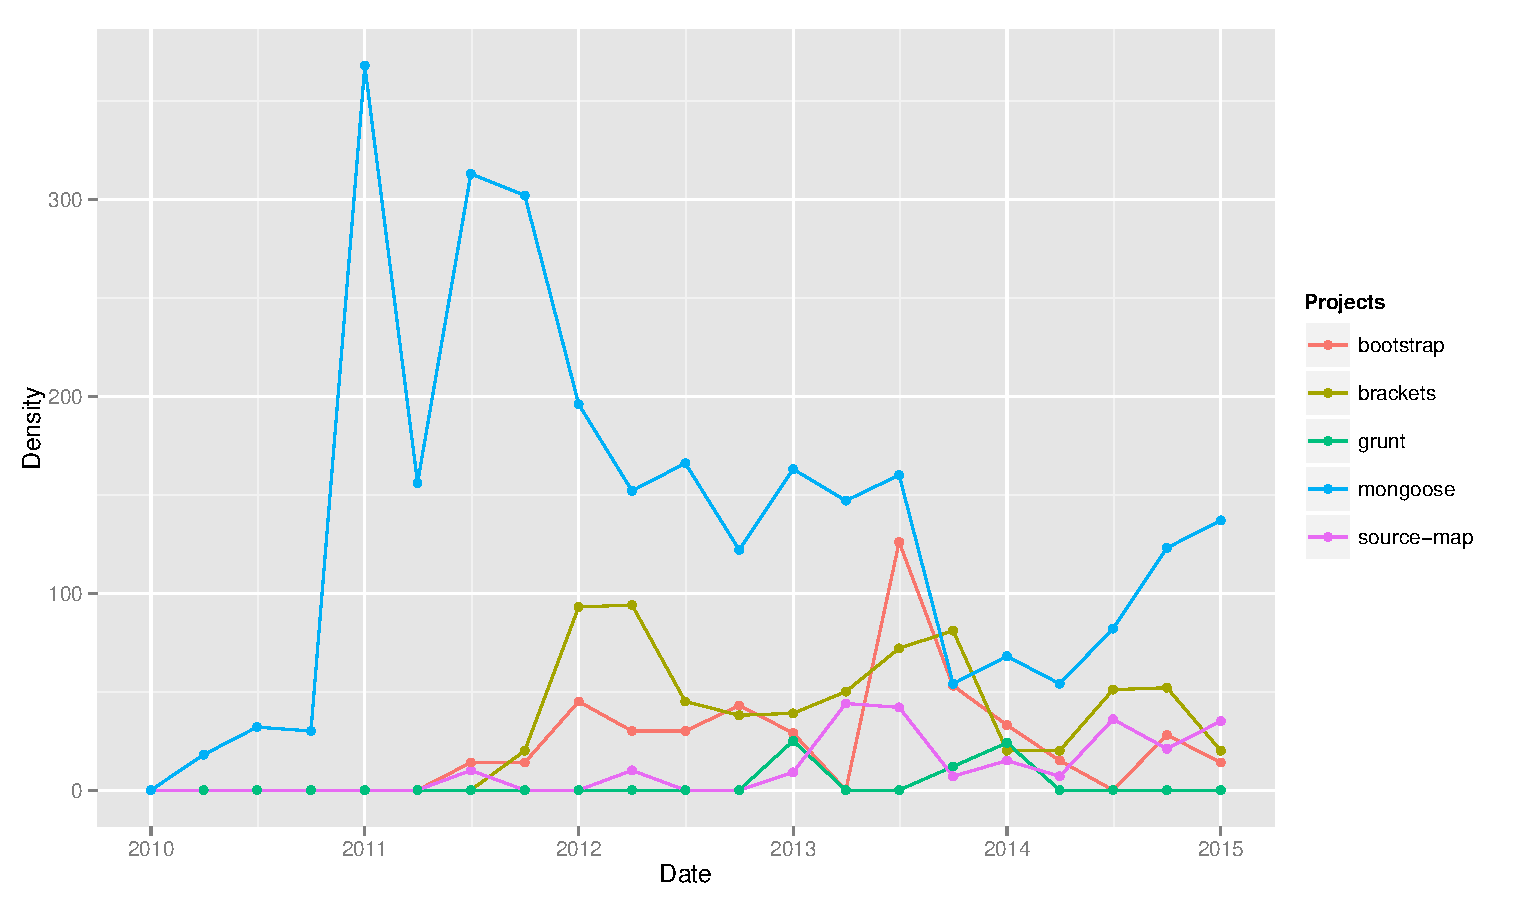
\includegraphics[width=90mm,scale=0.5]{figures/function_density}
 \end{figure}


\par
Having comments as one of the artifacts that can improve the readability of source code we examined it as metric of evolution.
Brackets has the most comment lines with having 63923 comment lines followed by Ember.js with 14698 comment lines. The least documented project is CoffeeScript with having only 124 lines of documentation. What makes the resuls interesting, is the fact that CoffeeScript starts with 836 lines of comments in the first release but in the last release we have only 124 lines of code. CoffeeScript and Grunt are the only projects that adapt this pattern, while all the other projects show growing trend in number of comments during evolution.  


\par
% developers_release